\chapter{需求建模 }
\section{数据流图}
\subsection{顶层数据流图}

顶层数据流图:
\begin{figure}[ht]
	\centering
    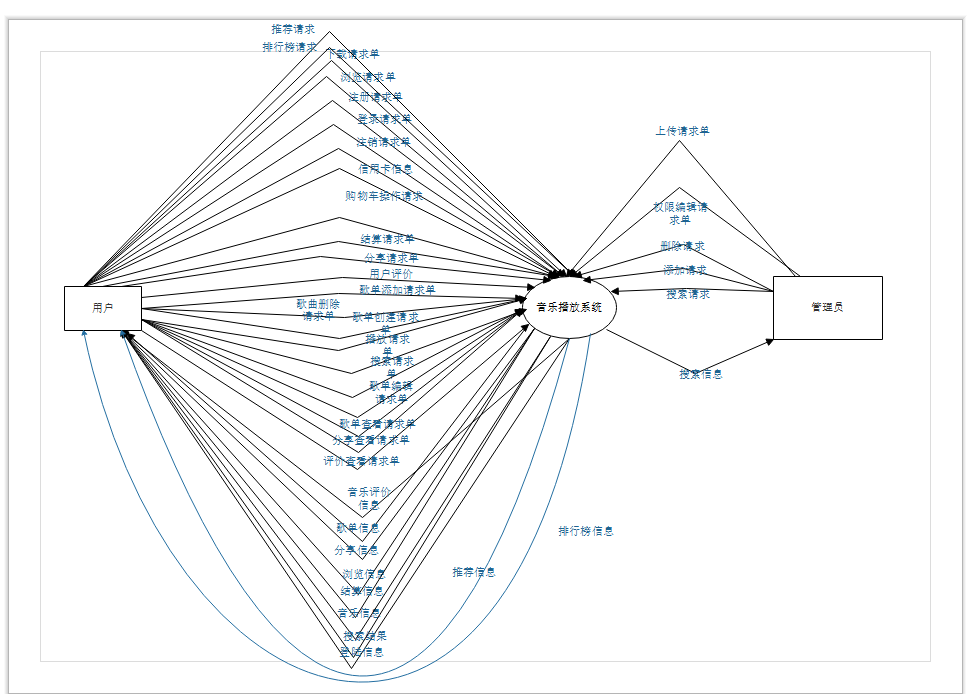
\includegraphics[width=15cm]{Top.png}
	\caption{顶层数据流图} \label{fig:figure3}
	\end{figure}

\subsection{0层数据流图}
0层数据流图:

\quad\\[\intextsep] 
  \begin{minipage}{\textwidth} 
    \centering 
    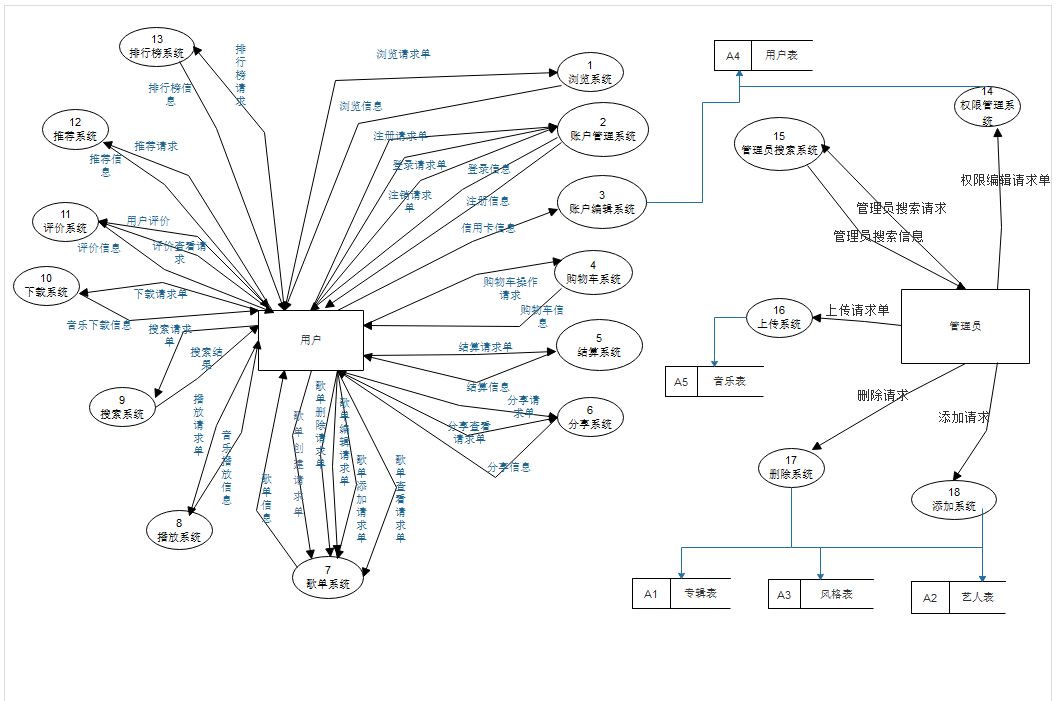
\includegraphics[width=6in]{0.png}% 
    \figcaption{0层数据流图} 
    \label{fig:non:float} 
  \end{minipage} 
  \quad\\[\intextsep] 

\subsection{1层数据流图}


\quad\\[\intextsep] 
  \begin{minipage}{\textwidth} 
    \centering 
    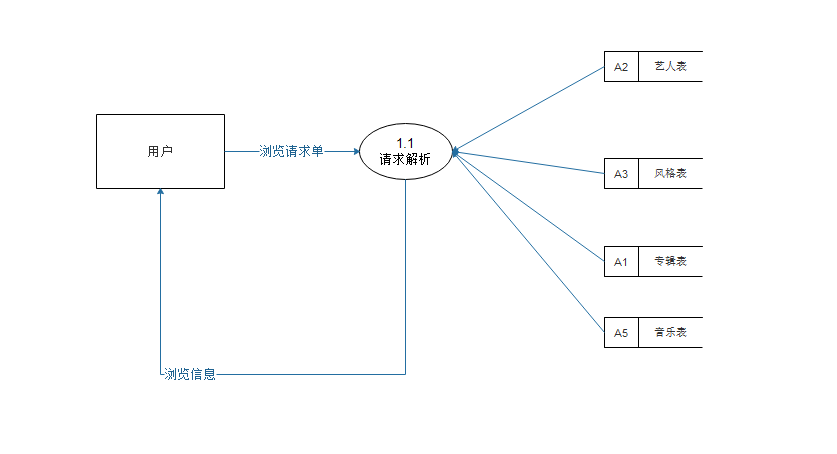
\includegraphics[width=6in]{101.png}% 
    \figcaption{数据流图1.1}
     \label{fig:non:float} 
  \end{minipage} 
  \quad\\[\intextsep] 


  
\quad\\[\intextsep] 
\begin{minipage}{\textwidth} 
  \centering 
  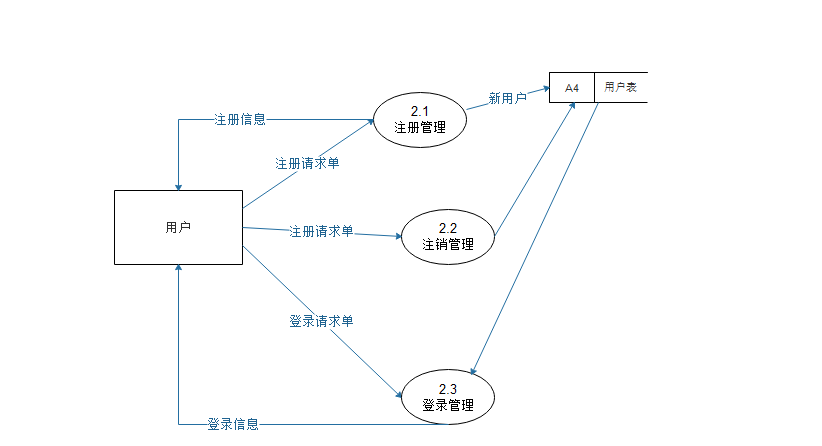
\includegraphics[width=6in]{102.png}% 
  \figcaption{数据流图1.2} 
  \label{fig:non:float} 
\end{minipage} 
\quad\\[\intextsep] 


\quad\\[\intextsep] 
\begin{minipage}{\textwidth} 
  \centering 
  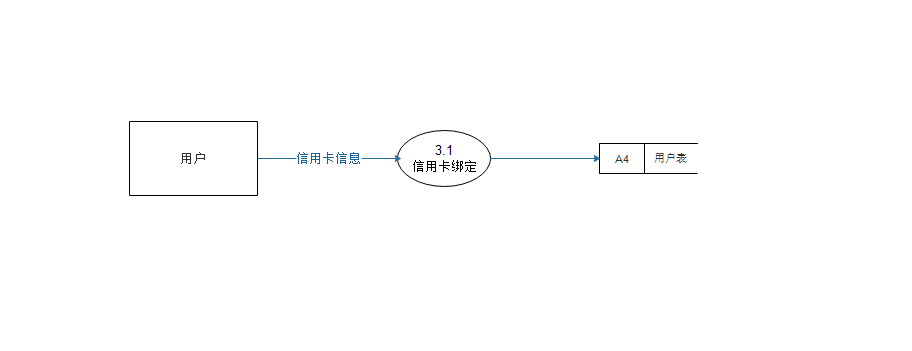
\includegraphics[width=6in]{103.png}% 
  \figcaption{数据流图1.3} 
  \label{fig:non:float} 
\end{minipage} 
\quad\\[\intextsep] 

\quad\\[\intextsep] 
\begin{minipage}{\textwidth} 
  \centering 
  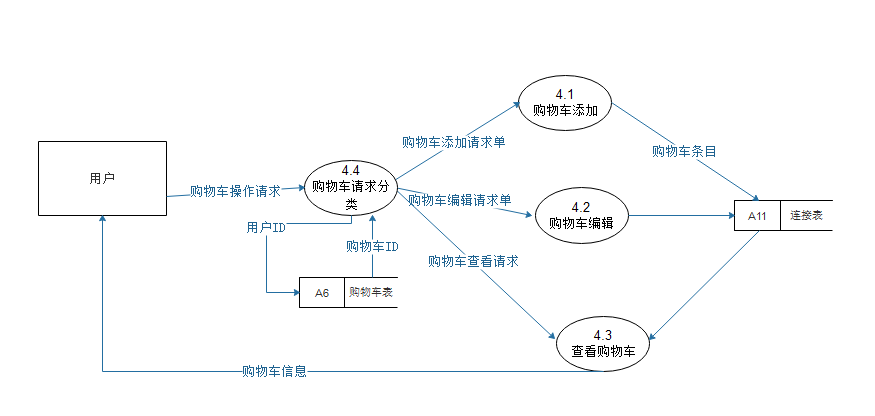
\includegraphics[width=6in]{104.png}% 
  \figcaption{数据流图1.4} 
  \label{fig:non:float} 
\end{minipage} 
\quad\\[\intextsep] 

\quad\\[\intextsep] 
\begin{minipage}{\textwidth} 
  \centering 
  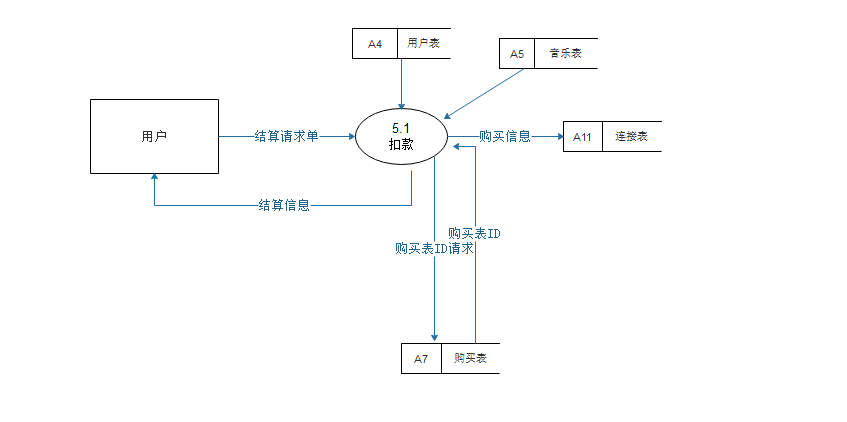
\includegraphics[width=6in]{105.png}% 
  \figcaption{数据流图1.5} 
  \label{fig:non:float} 
\end{minipage} 
\quad\\[\intextsep] 

\quad\\[\intextsep] 
\begin{minipage}{\textwidth} 
  \centering 
  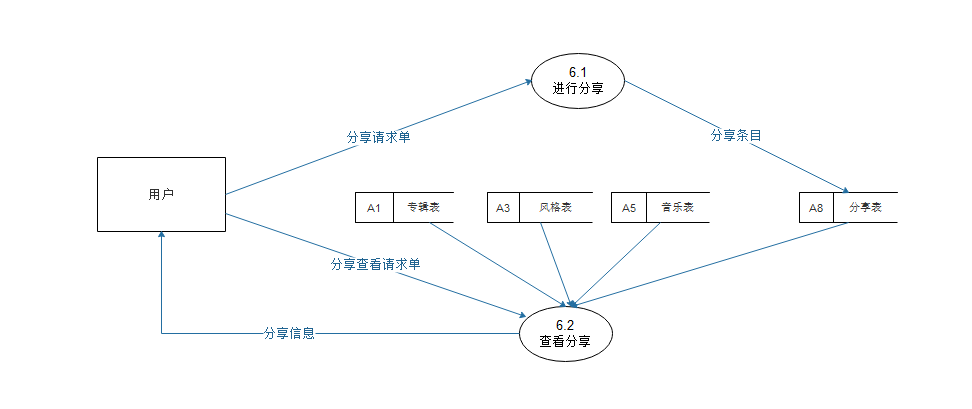
\includegraphics[width=6in]{106.png}% 
  \figcaption{数据流图1.6} 
  \label{fig:non:float} 
\end{minipage} 
\quad\\[\intextsep] 
 
\quad\\[\intextsep] 
\begin{minipage}{\textwidth} 
  \centering 
  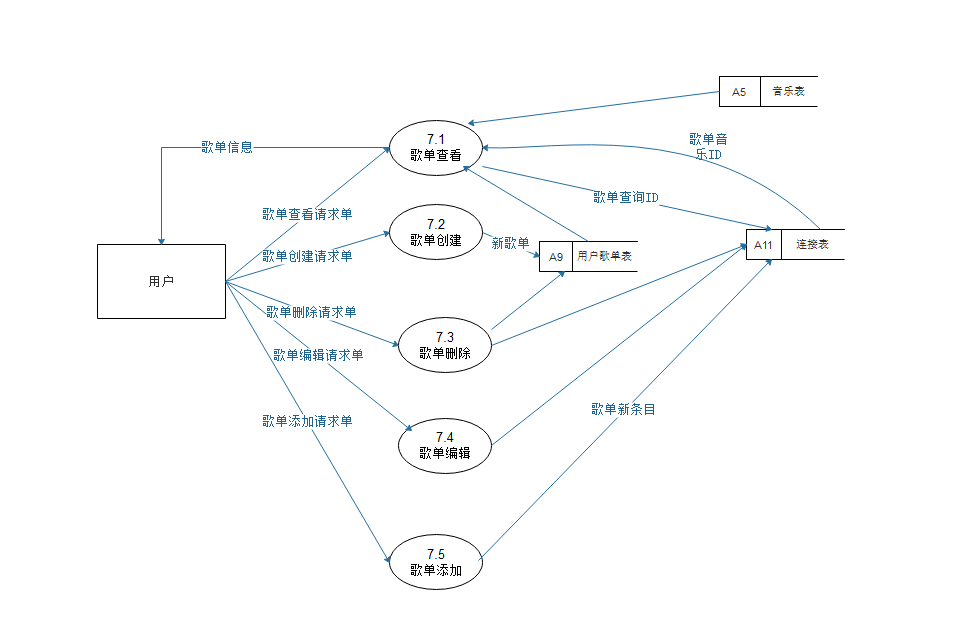
\includegraphics[width=6in]{107.png}% 
  \figcaption{数据流图1.7} 
  \label{fig:non:float} 
\end{minipage} 
\quad\\[\intextsep] 
    
\quad\\[\intextsep] 
\begin{minipage}{\textwidth} 
  \centering 
  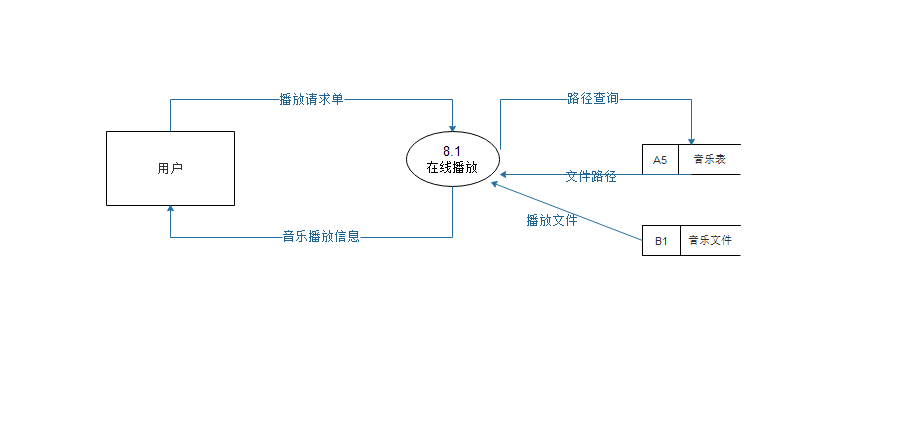
\includegraphics[width=6in]{108.png}% 
  \figcaption{数据流图1.8} 
  \label{fig:non:float} 
\end{minipage} 
\quad\\[\intextsep] 
       
\quad\\[\intextsep] 
\begin{minipage}{\textwidth} 
  \centering 
  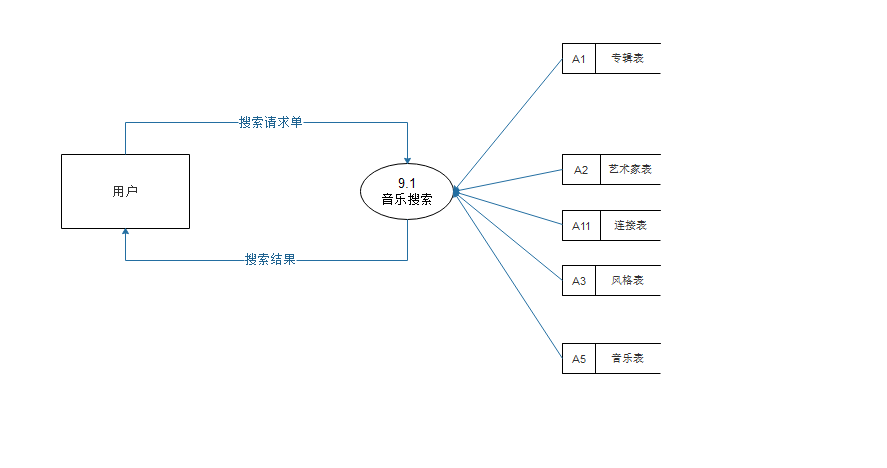
\includegraphics[width=6in]{109.png}% 
  \figcaption{数据流图1.9} 
  \label{fig:non:float} 
\end{minipage} 
\quad\\[\intextsep] 

\quad\\[\intextsep] 
\begin{minipage}{\textwidth} 
  \centering 
  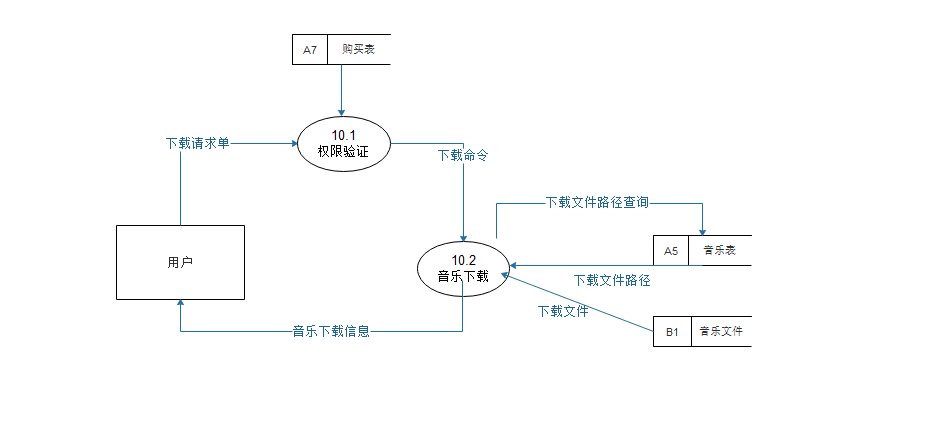
\includegraphics[width=6in]{1010.png}% 
  \figcaption{数据流图1.10} 
  \label{fig:non:float} 
\end{minipage} 
\quad\\[\intextsep] 
  
\quad\\[\intextsep] 
\begin{minipage}{\textwidth} 
  \centering 
  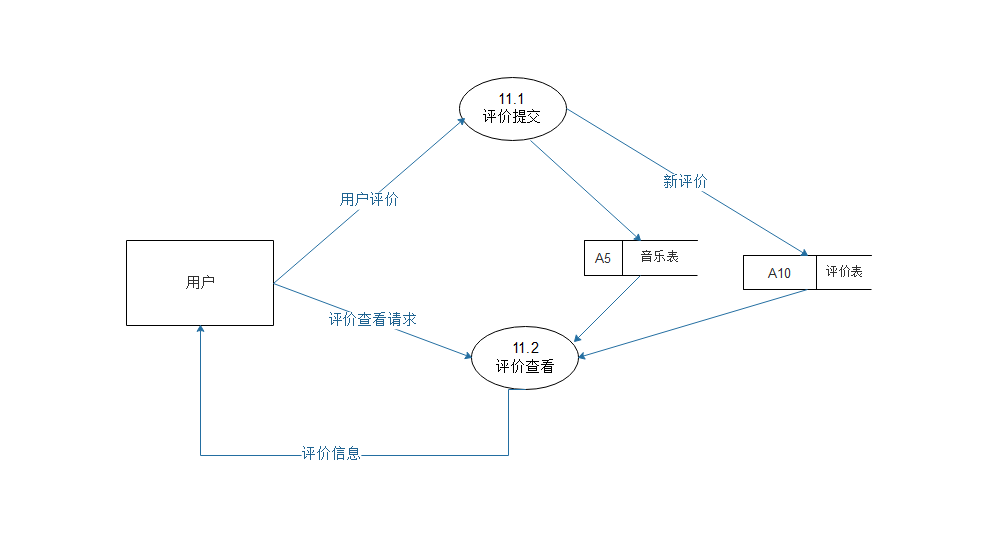
\includegraphics[width=6in]{1011.png}% 
  \figcaption{数据流图1.11} 
  \label{fig:non:float} 
\end{minipage} 
\quad\\[\intextsep] 

\quad\\[\intextsep] 
\begin{minipage}{\textwidth} 
  \centering 
  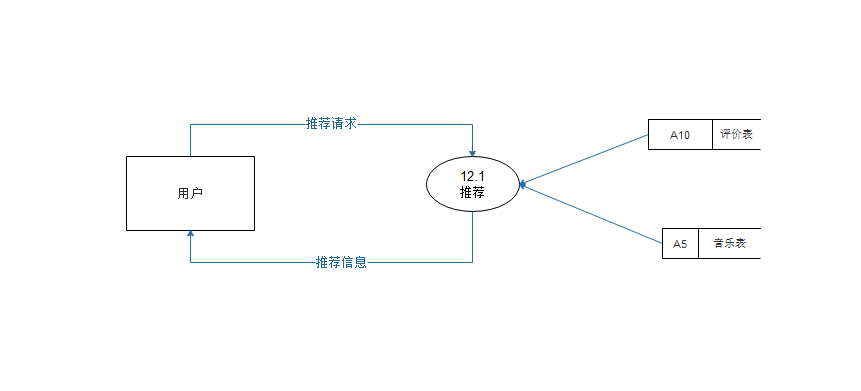
\includegraphics[width=6in]{1012.png}% 
  \figcaption{数据流图1.12} 
  \label{fig:non:float} 
\end{minipage} 
\quad\\[\intextsep] 

    
\quad\\[\intextsep] 
\begin{minipage}{\textwidth} 
  \centering 
  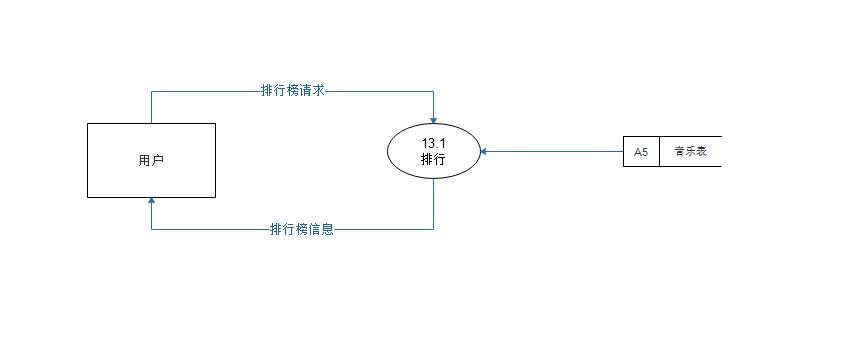
\includegraphics[width=6in]{1013.png}% 
  \figcaption{数据流图1.13} 
  \label{fig:non:float} 
\end{minipage} 
\quad\\[\intextsep] 
          
\quad\\[\intextsep] 
\begin{minipage}{\textwidth} 
  \centering 
  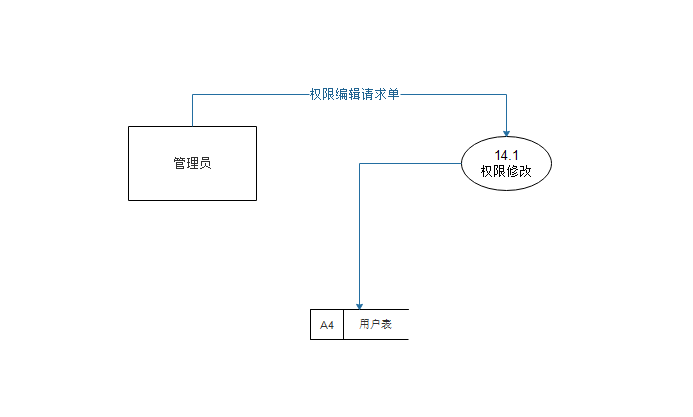
\includegraphics[width=6in]{1014.png}% 
  \figcaption{数据流图1.14} 
  \label{fig:non:float} 
\end{minipage} 
\quad\\[\intextsep] 
            
\quad\\[\intextsep] 
\begin{minipage}{\textwidth} 
  \centering 
  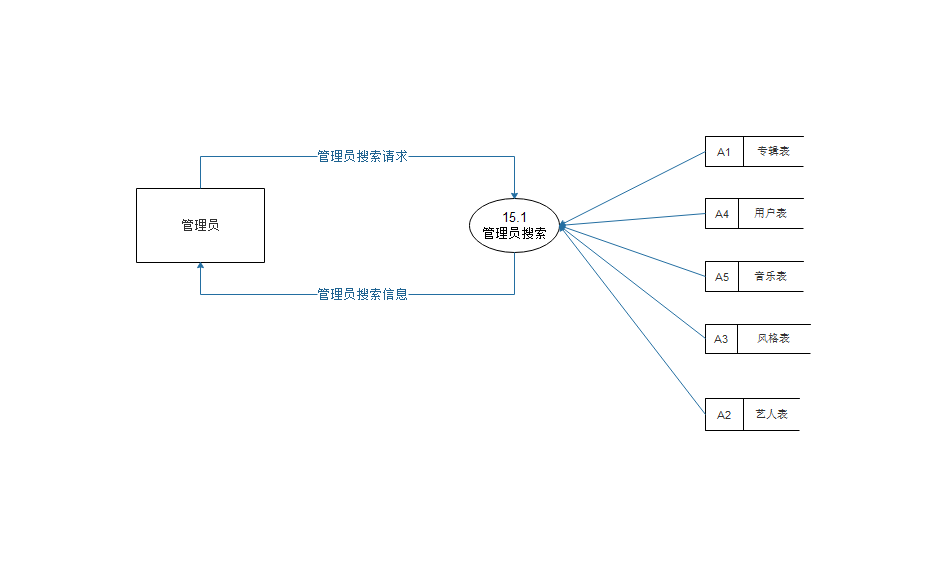
\includegraphics[width=6in]{1015.png}% 
  \figcaption{数据流图1.15} 
  \label{fig:non:float} 
\end{minipage} 
\quad\\[\intextsep] 
   
\quad\\[\intextsep] 
\begin{minipage}{\textwidth} 
  \centering 
  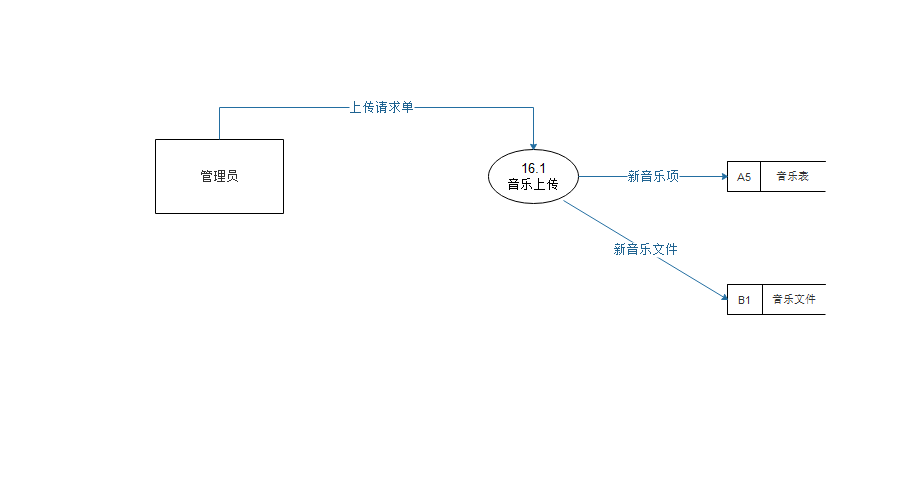
\includegraphics[width=6in]{1016.png}% 
  \figcaption{数据流图1.16} 
  \label{fig:non:float} 
\end{minipage} 
\quad\\[\intextsep] 
   
\quad\\[\intextsep] 
\begin{minipage}{\textwidth} 
  \centering 
  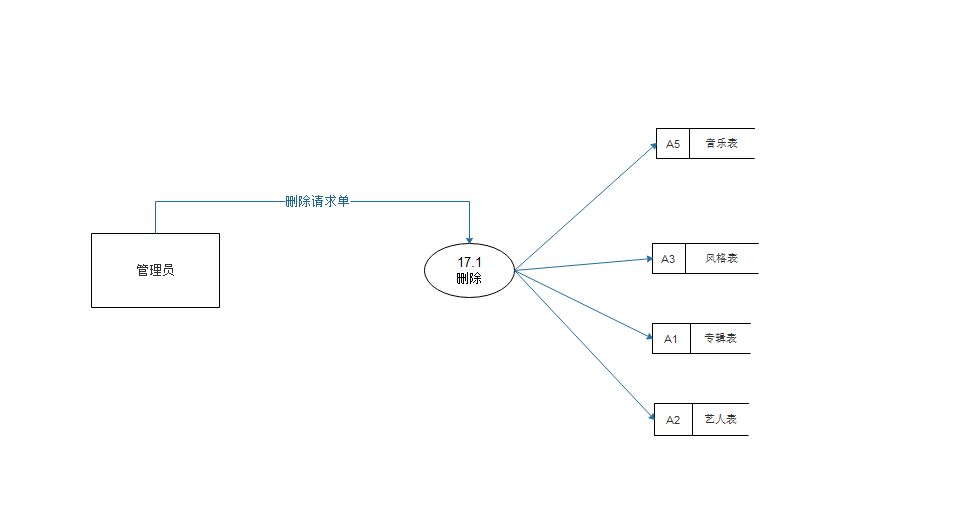
\includegraphics[width=6in]{1017.png}% 
  \figcaption{数据流图1.17} 
  \label{fig:non:float} 
\end{minipage} 
\quad\\[\intextsep] 
   
\quad\\[\intextsep] 
\begin{minipage}{\textwidth} 
  \centering 
  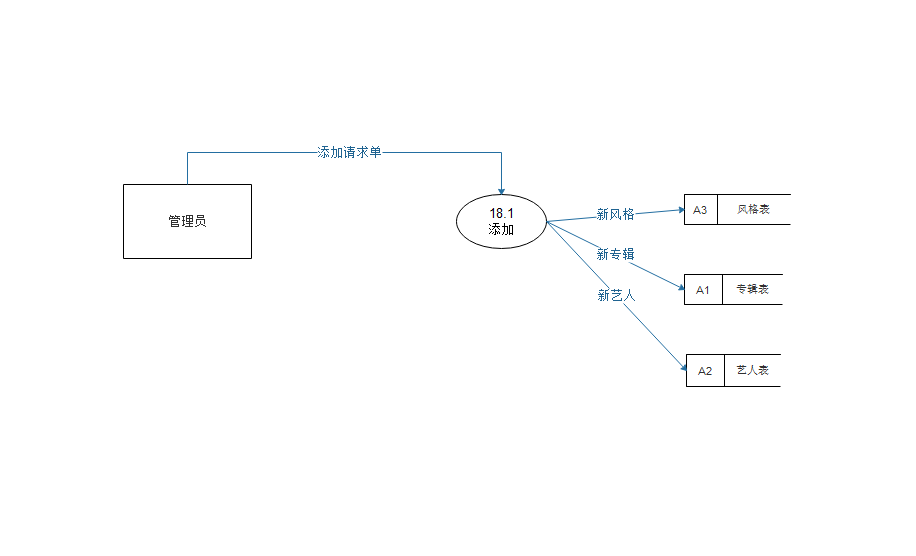
\includegraphics[width=6in]{1018.png}% 
  \figcaption{数据流图1.18} 
  \label{fig:non:float} 
\end{minipage} 
\quad\\[\intextsep] 



\section{数据字典}
\subsection{数据流说明}
\subsubsection{浏览请求单}

包括浏览的类别信息,是专辑,风格还是艺术家,以及专辑ID或者风格ID或者艺术家ID。
类别是整型,ID是长度1-20的Unicode字符串.
由用户发出到服务器.

\subsubsection{浏览信息}

根据浏览请求的不同,浏览信息可能是以下三种之一:
某个类别的音乐,
某张专辑中的音乐,
某个艺术家的所有专辑。
发送音乐会发送音乐ID,音乐名和音乐文件的路径url。
发送专辑会发送专辑名和专辑ID。

由服务器发送到用户。
\subsubsection{注册请求单}

包括新注册用户的用户名和密码
分别都是长度1-20的Unicode字符串.
由用户发送给服务器。

\subsubsection{注销请求单}

包括要注销的用户的用户ID和当前IP地址.

\subsubsection{登录请求单}

包括要登录的用户的用户ID,输入的密码和当前IP地址.

\subsubsection{注册信息}

一个成功通知或错误代码,都是长度1-20的Unicode字符串

\subsubsection{新用户}

一条新的用户条目,包括用户ID,用户名,用户密码和用户权限,其他属性为空。

\subsubsection{登录信息}

一个成功通知或错误代码。

\subsubsection{信用卡信息}

用户的用户ID和信用卡号,信用卡号是长为20的Unicode字符串.

\subsubsection{购物车操作请求}

包括用户ID,音乐ID(可为空)和操作类别(整型变量1或2或0)

\subsubsection{用户ID}

用户的ID。

\subsubsection{购物车ID}

购物车的ID,一个1-20的Unicode字符串。

\subsubsection{购物车添加请求单}

包括购物车ID和要加入购物车的音乐ID。

\subsubsection{购物车编辑请求单}
包括购物车ID和要从购物车中删去的音乐ID。

\subsubsection{购物车查看请求}
仅包括购物车ID。

\subsubsection{购物车条目}

一个新添加的购物车条目,包括购物车ID和音乐ID。

\subsubsection{购物车信息}
包括一个购物车的所有音乐的ID和音乐名,价格。

\subsubsection{结算请求单}

包括用户ID和要购买的所有音乐的ID。

\subsubsection{购买表ID请求}

一个购买表ID查询请求,包括用户ID。

\subsubsection{购买表ID}

一个用户的购买表ID。

\subsubsection{购买信息}

要插入购买表的一个条目,包括购买表ID和音乐ID。

\subsubsection{结算信息}

包括用户ID,购买的音乐ID以及一个通知(成功的消息或者错误码)

\subsubsection{分享请求单}

包括分享者UID,接受者UID,分享的类型(整型,表示是单曲,专辑还是用户歌单),和对应的ID(音乐表的ID或者音乐ID)以及分享时间(data型变量)

\subsubsection{分享查看请求单}

包括用户ID。

\subsubsection{分享信息}

包括某个用户收到的分享内容,包括分享者的UID,分享的类型(单曲,专辑还是用户歌单)以及对应的ID。

\subsubsection{分享条目}

要插入分享表的一个新条目,在分享信息的基础上增加了分享时间。

\subsubsection{歌单查看请求单}

包括歌单的ID,歌单ID是一个1-20的Unicode字符串,在数据库中唯一标识了一个用户歌单。

\subsubsection{歌单编辑请求单}

包括歌单的ID,提出申请的用户的ID,以及被删除的音乐的ID。

\subsubsection{歌单添加请求单}

包括歌单的ID,提出申请的用户的ID,以及被添加的音乐的ID。

\subsubsection{歌单删除请求单}

包括被删除的歌单的ID,提出申请的用户的ID。

\subsubsection{歌单创建请求单}

包括用户ID,被创建的歌单名和描述。

\subsubsection{歌单信息}

包括歌单的ID,歌单的名字(一个字符串),以及歌单中所有音乐的ID和名字。

\subsubsection{新歌单}

一个新的歌单条目,包括用户ID,歌单ID,歌单名和歌单描述(一个1-20的Unicode字符串)

\subsubsection{歌单新条目}

连接一个歌单和一首音乐的条目,包括歌单ID和音乐ID。

\subsubsection{歌单查询ID}

歌单ID

\subsubsection{歌单音乐ID}

若干音乐ID。

\subsubsection{播放请求单}

包括提出申请的用户的ID和要播放的音乐的ID。


\subsubsection{路径查询}

包括音乐ID。

\subsubsection{文件路径}

文件路径是音乐文件在服务器中的存储位置,是一个url。

\subsubsection{播放文件}

被播放的音乐文件。

\subsubsection{音乐播放信息}

用户在线播放所需要的所有文件信息。

\subsubsection{搜索请求单}

包括可选的风格名,专辑名,艺术家名和音乐名等信息,以上信息都是Unicode字符串形式.

\subsubsection{搜索结果}

为用户返回的所有搜索到的音乐的ID和名称。


\subsubsection{下载请求单}

包括用户ID和要下载的音乐ID。

\subsubsection{下载命令}

包括一个bool型变量表示权限认证成功与否,用户ID和要下载的音乐ID。

\subsubsection{下载路径查询}

音乐ID。

\subsubsection{下载文件路径}

文件路径是音乐文件在服务器中的存储位置,是一个url。

\subsubsection{下载文件}

被下载的音乐文件。

\subsubsection{音乐下载信息}

一个错误码或者用户所下载的音乐文件的下载链接。

\subsubsection{用户评价}

包括用户ID,音乐ID,用户评分(整型,取值为1-10)和评价内容(1-50的Unicode字符串)

\subsubsection{评价查看请求}

音乐ID。

\subsubsection{评价信息}

包括音乐ID,音乐名,评价人数(长整型),平均分(浮点型,取值范围为1-10),

\subsubsection{新评价}

一个新的评价条目,包括用户ID,音乐ID,用户评分(1-10的整数)和评价内容(可以为空)

\subsubsection{推荐请求}

用户ID。

\subsubsection{推荐信息}

包含向用户推荐的音乐的歌曲的ID。

\subsubsection{排行榜请求}

仅包含一个命令码表明是排行榜请求。

\subsubsection{排行榜信息}

包含排行榜上的音乐以及次序.

\subsubsection{权限编辑请求单}

包含申请用户ID,被修改用户ID和目标权限信息(整型)

\subsubsection{管理员搜索请求}

包含搜索者ID,以及可选的风格名,专辑名,艺术家名和音乐名等信息,以上信息都是Unicode字符串形式.

\subsubsection{管理员搜索信息}

为管理员返回的搜索到的音乐表ID或音乐ID或艺人ID。

\subsubsection{上传请求单}

包括上传者ID,上传的音乐文件,以及上传音乐的所有信息,艺术家ID,专辑ID,音乐名,评价人数,平均分,总播放次数,风格,价格

\subsubsection{新音乐项}

一个新的音乐项目,包括:音乐ID,艺人ID,专辑ID,音乐名,评价人数,平均分,总播放次数,风格ID,价格

\subsubsection{新音乐文件}

刚上传的音乐文件

\subsubsection{删除请求单}

包括删除的类别(整型),和要被删除的对象的ID
可以被删除的对象包括:音乐,专辑,风格和艺人。

\subsubsection{添加请求单}


包括添加的类别(整型),和要被添加的对象的所有信息,具体信息参考第六章数据库说明。
可以被添加的对象包括:专辑,风格和艺人。

\subsection{数据存储说明}
\subsubsection{A1:专辑表}

所有专辑的信息,存在于数据库中,每一个专辑的内容参考第六章数据库说明:
TID,Tname,描述(char),YID(外键)
即专辑ID,专辑名,专辑描述,专辑所属艺人ID
专辑表是音乐表表的子类

\subsubsection{A2:艺人表}

所有艺人的信息,存在于数据库中,每一个艺人的内容如下:
YID(主键),Yname,性别,生日
即艺人的ID,和姓名、性别,生日

\subsubsection{A3:风格表}

所有风格的信息,存在于数据库中,每一个风格的内容如下:
TID,Tname,描述(char)
即风格表ID,风格名,风格描述
风格表是音乐表表的子类

\subsubsection{A4:用户表}
所有用户的信息,存在于数据库中,每一个用户的内容如下:
UID(主键),Uname,password,权限(普通用户,管理员),信用卡号,分享状态,当前IP
其中,权限是int型变量,分享状态是bool变量,表示用户当前是否有未读分享信息,当前IP记录已登录用户当前的IP,若离线,则IP为NULL

\subsubsection{A5:音乐表}
所有音乐的信息,存在于数据库中,每一个音乐的内容如下:
MID(主键),YID(外键),TID(外键),Mname,评价人数,平均分,总播放次数,风格ID,价格
其中MID是音乐的ID,YID是艺人ID,TID是专辑ID

\subsubsection{A6:购物车表}
所有购物车的信息,存在于数据库中,每一个购物车内容如下:
UID(主键,外键),TID
UID是用户ID,TID是购物车的ID,购物车是一个音乐表,每个用户只有一个购物车
购物车表是音乐表表的子类

\subsubsection{A7:购买表}
所有用户的购买信息,存在于数据库中,每一个购买内容如下:
UID(主键,外键),TID
UID是用户ID,TID是购买的ID,购买是一个音乐表,每个用户只有一个购买
购买表是音乐表表的子类

\subsubsection{A8:分享表}

所有的购买信息,存在于数据库中,每一个分享条目的内容如下:
RUID(主键,外键),CUID(外键),time,类别,ID(MID或TID)
其中,RUID是接受分享者的UID,CUID是分享者的UID,time是分享建立的时间

\subsubsection{A9:用户歌单表}

所有用户歌单的信息,存在于数据库中,每一个用户歌单的内容如下:
UID(外键),TID(主键),Tname,描述(char),TAG1,TAG2,TAG3
其中TAG是整数类型,是一个标签
用户歌单表是音乐表表的子类


\subsubsection{A10:评价表}

所有评价的信息,存在于数据库中,每一条评价的内容如下:
UID(主键),MID(主键),评分,评价内容(可以为空)

\subsubsection{A11:连接表}

所有音乐表表和音乐表的对应关系,连接表内容参见第六章数据库说明:
因为音乐表和音乐之间是多对多的关系,所以需要一个连接表来表示各个音乐表和音乐的关系,连接表的内容是:TID和MID,即表ID和音乐ID


\subsubsection{B1:音乐文件}

所有的音乐文件,音乐文件存在于服务器上,每一个文件都有一个文件路径,文件路径存在音乐表中。

\subsection{加工说明}
\subsubsection{1.1 请求解析}

根据用户发来的浏览请求单的类型,使用ID到对应的数据库的表中获得对应的条目的信息。作为浏览信息发回给用户。

\subsubsection{2.1 注册管理 }

根据用户发来的请求单中的用户名和密码,为用户分配一个UID和权限,将新用户写入用户表中。
如果注册成功,将成功消息发回给用户,否则发回错误码.

\subsubsection{2.2 注销管理 }

根据用户发来的注销请求单中的ID,在用户表中将对应用户条目的IP地址设为NULL。

\subsubsection{2.3 登录管理 }

根据用户发来的登录请求单中的用户ID和密码,在用户表中进行对比,如果匹配,则登录成功,将用户IP地址设为当前IP地址。
如果登录成功,将成功消息发回给用户,否则发回错误码.

\subsubsection{3.1 信用卡绑定 }

根据用户发来的信用卡信息中的ID和信用卡号,把信用卡信息写入用户表中对应条目.

\subsubsection{4.1 购物车添加 }

根据购物车添加请求单中的购物车ID,在连接表中插入购物车ID和音乐ID。

\subsubsection{4.2 购物车编辑 }

根据购物车编辑请求单中的购物车ID,在连接表中删除购物车ID和音乐ID对应的条目.

\subsubsection{4.3 查看购物车 }

根据购物车查看请求中的购物车ID,根据购物车ID和连接表中信息,在音乐表中选择所有音乐条目返回给用户。

\subsubsection{4.4购物车请求分类}

根据购物车操作请求中的用户ID去购物车表中查找用户的购物车ID,然后根据请求种类决定调用添加,编辑还是查看功能,将购物车ID,音乐ID发送到对应的加工。

\subsubsection{5.1 扣款 }

根据用户发来的结算请求单中的用户ID,在用户表中找到对应的信用卡信息,根据用户发来的音乐ID,在音乐表中得到对应的音乐价格,然后从用户信用卡中扣款。
如果扣款成功,在在购买表中查询用户的购买表ID,将购买表ID和购买的音乐ID组成购买信息,将购买信息插入连接表。
如果扣款成功,发回成功消息和对应音乐信息,否则发回错误码。

\subsubsection{6.1进行分享}

将用户发来的分享请求单分享者ID,接收者ID,分享类型和分享内容ID与服务器当前时间一起作为一个条目写入分享表。

\subsubsection{6.2查看分享}

根据用户发来的分享查看请求单中的UID,在分享表中查找所有对应的条目,根据每个条目对应的分享内容分别在专辑表,风格表和音乐表中进行查找,将查找内容作为分享信息返回给用户。

\subsubsection{7.1歌单查看}

根据用户发来的歌单查看请求单中的歌单ID在连接表中查找对应的音乐ID,根据从连接表中查到的音乐ID在音乐表中中查找对应的音乐。
将歌单ID,音乐ID,歌单相关信息和音乐相关信息都作为歌单信息发送给用户。


\subsubsection{7.2歌单创建}

根据用户发来的歌单创建请求单中的UID为用户分配一个歌单ID,结合请求单中的歌单名和描述,在用户歌单表中插入一个新的歌单条目。


\subsubsection{7.3歌单删除}

根据用户发来的歌单删除请求单中的UID,和歌单ID,在用户歌单表中删除对应的歌单ID,并在连接表中删除对应的所有条目。

\subsubsection{7.4歌单编辑}

根据用户发来的歌单编辑请求单中的歌单ID和音乐ID,在连接表中删除对应的条目。

\subsubsection{7.5歌单添加}

根据用户发来的歌单添加请求单中的歌单ID和音乐ID,在连接表中插入对应的条目。

\subsubsection{8.1在线播放}

根据用户发来的播放请求单中的音乐ID在音乐表中进行查询,得到音乐文件路径,根据路径得到音乐文件,包装成音乐播放信息发给用户。

\subsubsection{9.1音乐搜索}

根据用户发来的搜索请求单中的风格名,专辑名,艺术家名或音乐名在对应的表中进行搜索,将搜索得到的音乐ID,音乐名作为搜索结果发给用户。

\subsubsection{10.1权限验证}

根据用户发来的下载请求单中的用户ID和音乐ID,在购买表中查找,如果找到了对应条目,表示用户购买了该音乐。
将权限验证结果和音乐ID一起发到音乐下载加工模块。

\subsubsection{10.2音乐下载}
根据权限验证结果和音乐ID进行下载,如果权限合法,则根据音乐ID在音乐表中搜索得到下载文件的路径,根据文件路径得到音乐文件,返回给用户。
如果权限验证失败,则返回给用户一个错误码。

\subsubsection{11.1评价提交}

根据用户评价中用户ID,音乐ID,用户评分和评价内容生成一个新的评价条目插入评价表中。
如果用户用户已经评价过该音乐,则将新评价条目更新到评价表中。
同时,更改音乐表中对应音乐的评价人数和平均分。
\subsubsection{11.2评价查看}

根据评价查看请求中的音乐ID,在评价表和音乐表中找到相应的条目,将评价人数,平均分和用户评价内容作为评价信息发回给用户。

\subsubsection{12.1推荐}

根据推荐请求中的用户ID,在评价表中找到用户的历史评价信息来判断用户的喜好,据此来形成推荐目录,将推荐的音乐的ID,音乐名的信息作为推荐信息发回给用户。

\subsubsection{13.1排行}

收到排行榜请求后,根据音乐表中的评分信息和播放次数信息生成两个排行榜作为排行榜信息发给用户。

\subsubsection{14.1权限修改}

根据权限编辑请求单中的被修改用户ID和目标权限信息来修改用户表中对应用户的权限信息。

\subsubsection{15.1管理员搜索}

根据管理员搜索请求中的风格名,专辑名,艺术家名,音乐名或用户名在对应的表中进行搜索,将搜索得到的信息发给管理员。

\subsubsection{16.1音乐上传}

根据上传请求单中的音乐文件分配一个路径,将文件存到该位置,为新的音乐分配一个ID,然后将ID,文件路径和上传请求单中的艺术家ID,专辑ID,音乐名,评价人数,平均分,总播放次数,风格,价格信息结合成为一个新的音乐条目插入音乐表中。

\subsubsection{17.1删除}

根据删除请求单中的删除类别和要删除的ID来删除对应表中的条目。

\subsubsection{18.1添加}

根据添加请求单中的类别信息来决定向哪个表中做插入操作。
向风格表中插入一个风格ID
或者向专辑表中插入一个专辑ID与艺术家ID组成的条目
或者向艺人表中插入一个由艺人ID,艺人姓名,性别(可选),生日(可选)组成的艺人条目。





